\documentclass[
	ngerman,
	ruledheaders=section,%Ebene bis zu der die Überschriften mit Linien abgetrennt werden, vgl. DEMO-TUDaPub
	class=report,% Basisdokumentenklasse. Wählt die Korrespondierende KOMA-Script Klasse
	thesis={type=master},% Dokumententyp Thesis, für Dissertationen siehe die Demo-Datei DEMO-TUDaPhd
	accentcolor=8c,% Auswahl der Akzentfarbe
	custommargins=false,% Ränder werden mithilfe von typearea automatisch berechnet
	marginpar=false,% Kopfzeile und Fußzeile erstrecken sich nicht über die Randnotizspalte
	%BCOR=5mm,%Bindekorrektur, falls notwendig
	parskip=half-,%Absatzkennzeichnung durch Abstand vgl. KOMA-Sript
	fontsize=11pt,%Basisschriftgröße laut Corporate Design ist mit 9pt häufig zu klein
%	logofile=example-image, %Falls die Logo Dateien nicht vorliegen
]{tudapub}


% Der folgende Block ist nur bei pdfTeX auf Versionen vor April 2018 notwendig
\usepackage{iftex}
\ifPDFTeX
	\usepackage[utf8]{inputenc}%kompatibilität mit TeX Versionen vor April 2018
\fi

%%%%%%%%%%%%%%%%%%%
%Sprachanpassung & Verbesserte Trennregeln
%%%%%%%%%%%%%%%%%%%
\usepackage[ngerman, main=english]{babel}
\usepackage[autostyle]{csquotes}% Anführungszeichen vereinfacht

% Falls mit pdflatex kompiliert wird, wird microtype automatisch geladen, in diesem Fall muss diese Zeile entfernt werden, und falls weiter Optionen hinzugefügt werden sollen, muss dies über
% \PassOptionsToPackage{Optionen}{microtype}
% vor \documentclass hinzugefügt werden.
\usepackage{microtype}
\usepackage{subfig}

%%%%%%%%%%%%%%%%%%%
%Literaturverzeichnis
%%%%%%%%%%%%%%%%%%%
\usepackage[style=ieee, backend=bibtex]{biblatex}
\bibliography{Sources.bib}


%%%%%%%%%%%%%%%%%%%
%Paketvorschläge Tabellen
%%%%%%%%%%%%%%%%%%%
%\usepackage{array}     % Basispaket für Tabellenkonfiguration, wird von den folgenden automatisch geladen
\usepackage{tabularx}   % Tabellen, die sich automatisch der Breite anpassen
%\usepackage{longtable} % Mehrseitige Tabellen
%\usepackage{xltabular} % Mehrseitige Tabellen mit anpassbarer Breite
\usepackage{booktabs}   % Verbesserte Möglichkeiten für Tabellenlayout über horizontale Linien

%%%%%%%%%%%%%%%%%%%
%Paketvorschläge Mathematik
%%%%%%%%%%%%%%%%%%%
%\usepackage{mathtools} % erweiterte Fassung von amsmath
%\usepackage{amssymb}   % erweiterter Zeichensatz
%\usepackage{siunitx}   % Einheiten
\usepackage{pgfplots}   % Plots
\usepackage{pgfplotstable}
\pgfplotsset{compat=1.5}
\usepgfplotslibrary{dateplot}
\usepackage{caption}
\usepackage{smartdiagram}

%Formatierungen für Beispiele in diesem Dokument. Im Allgemeinen nicht notwendig!
\let\file\texttt
\let\code\texttt
\let\tbs\textbackslash

\usepackage{pifont}% Zapf-Dingbats Symbole
\newcommand*{\FeatureTrue}{\ding{52}}
\newcommand*{\FeatureFalse}{\ding{56}}

\begin{document}

\Metadata{
	title=Pod Autoscaling in Kubernetes Cluster,
	author=Angelina Horn
}

\title{Pod Autoscaling in Kubernetes Cluster}
\author[]{Angelina Horn}%optionales Argument ist die Signatur,
\birthplace{Bonn}%Geburtsort, bei Dissertationen zwingend notwendig
\reviewer{Prof. Dr. Felix Wolf \and Dr. Hamid Mohammadi Fard}%Gutachter

%Diese Felder erden untereinander auf der Titelseite platziert.
%\department ist eine notwendige Angabe, siehe auch dem Abschnitt `Abweichung von den Vorgaben für die Titelseite'
\department{inf} % Das Kürzel wird automatisch ersetzt und als Studienfach gewählt, siehe Liste der Kürzel im Dokument.
\group{Parallel Programming}

\submissiondate{\today}
\examdate{\today}

%	\tuprints{urn=1234, printid=12345, doi=10.25534/tuprints-1234}
%	\dedication{Für alle, die \TeX{} nutzen.}

\maketitle

\affidavit[digital] %falls eine rein digitale Abgabe vorgesehen ist.

\tableofcontents

%%%%%%%%%%%%%%%%%%%
%Inhalt
%%%%%%%%%%%%%%%%%%%
\chapter{Introduction}
% Motivation
\section{Motivation}
Lately microservice architecture is gaining popularity especially among developers \cite{alshuqayran2016systematic}. The
microservice architecture describes a new and highly flexible way of application architecture and
deployment. For this approach an application gets split into smaller but independent chunks called
microservices. The created microservices will be deployed, for example as docker containers in a
server cluster. These clusters will often not be maintained or owned by the applications developer
but rather by an enterprise cloud provider like Google or Amazon. Microservices that belong to
one deployment can communicate between one another via lightweight API interfaces e.g. REST.\\
\newline
Applications will have a dynamic load based on several possible reasons such as daytime and
workload \cite{villamizar2015evaluating}. This load however is not distributed equally among all microservices. Therefore, it
is necessary to be able to scale the microservices while they are under load in order to maintain
performance of the whole application. Additionally, because of limited and costly resources, one
wants to use only the minimal amount of resources that are necessary to sustain performance.\\
\newline
This can be achieved via automatic scaling \cite{rossi2019horizontal}. Automatic scaling describes a mechanism which
periodically monitors every resource of a microservice, determines if and how a container should
be scaled based on metrics defined by the developer and executes the scaling automatically.
Because all these described architectures and ways of deployment are rather new there is room
for research and improvement regarding this topic.\\
\newpage
% Objective
\section{Objective}
The objective of this thesis is mainly to implement a machine learning process as part of a fully
automatic process, that produces a performance model of a docker container application, which
on one hand determines the scaling technique (vertically, horizontally or both) and on the other
hand how much and when to scale with the goal of not exceeding a given maximum response time.\\
Therefore the implementation can be divided into three separated goals (see \ref{fig:overview}):
\begin{enumerate}
\item The design of a graphical user interface which will be the single interaction point of the user. 
\item The development of a machine learning algorithm which takes performance data of a microservice as an input and produces a performance model of this microservice as a result. 
\item The implementation of a control script which connects the graphical user interface, the machine learning algorithm and Kubernetes. 
\end{enumerate}

The combination of these three goals will result in the above described fully automated process. Which will start with the input of the microservice docker image from the user and result in a fully deployed and auto-scaled microservice in a given Kubernetes cluster.
\newpage
%%%%%%%%%%%%%%%%%%%
% Background
%%%%%%%%%%%%%%%%%%%
\chapter{Background}
In this chapter of the thesis, basic topics of which their understanding is necessary, will be pointed out and explained. These topics are Microservices, Kubernetes and Autoscaling. Furthermore two applications that play an important role in this thesis called OctoScan and Extra-P will be presented. These topics will build the foundation and background needed for in this thesis following approaches, research and statements.
% Microservices
\section{Microservices}
The term "microservice" was first introduced by James Lewis in a conference \cite{lewis2012microservices}. It describes an application architecture which is characterized by subdivided applications, that communicate with each other trough lightweight interfaces.\\ 
Each of these applications has a single responsibility or task and is deployed independently. This means that each of these microservices can be implemented in a different programming language and can be deployed on an entirely different operating system on a different server as long as they share a common interfaces and are able to communicate with each other trough it. James Lewis describes this approach as "[...] rooted in the the Unix Philosophy of small and simple" \cite{lewis2012microservices}.\\

On one hand this architecture offers several advantages compared to the monolithic application architecture which was popular prior.
First and foremost it provides modularity which is highly beneficial regarding code complexity as well as team coordination \cite{dragoni2017microservices}. The introduction phase of new programmers is highly decreased as well as the possibilities to work on different parts of the overall application at the same time.\\
Secondly, this kind of architecture makes it possible to incrementally upgrade an application and therefore possibly to reduce time to market \cite{dragoni2017microservices}. Certain parts of the application can be updated independently from the other microservices regarding not only the application code itself but also its dependencies such as libraries and environments. This way the so called "dependency hell" \cite{merkel2014docker} which many monolithic applications suffer from can be avoided.\\
Furthermore microservices are more resistant to failure due to their containerized existence. If one microservice fails it does not necessary lead to the failure of the whole application. Additionally this failed microservice can be easily restarted in a short amount of time because of its lightweight nature.\\
Last but not least, microservices introduce a new capability of scaling \cite{dragoni2017microservices, namiot2014micro}. Regarding the application, each microservice is under inconsistent load and can be scaled individually. This allows optimal usage of resources in dependency of desired performance and costs.\\

On the other hand this architecture brings certain disadvantages.
One major disadvantage is the time it costs to convert any application in several microservices \cite{dragoni2017microservices}. This time should not be underestimated but can also bring major benefits as stated above.
Another disadvantage is the complexity of the deployment \cite{dragoni2017microservices}. Today there are several ways to deploy microservices including the use of Jenkins\footnote{https://www.jenkins.io} or lately the use of orchestral cluster tools such as Docker Swarm\footnote{https://docs.docker.com/engine/swarm} and Kubernetes\footnote{https://kubernetes.io}.\\
% Kubernetes
\section{Kubernetes}
The term Kubernetes gained a lot of popularity over the past five years (see figure \ref{fig:google-trends}). It is the name of a orchestral tool for containerized applications, originally designed by Google and now owned by the Cloud Native Computer Foundation\footnote{https://www.cncf.io}. Its capabilities include deployment, scaling and monitoring of containerized microservices in clusters. These clusters can be hosted in a public or private cloud.\\
% Begin Plot
\begin{figure}[h]
\label{fig:google-trends}
\centering
\resizebox{0.7\textwidth}{!}{
\begin{tikzpicture}
\begin{axis}[
date coordinates in = x,
xticklabel = {\year},
xlabel = {Year},
stack plots = y,
ylabel =  {Interest},
ylabel style={yshift = 10pt},
ymin = 0,
	] 
\addplot table [smooth, mark=none, x = Monat, y = Kubernetes] {data/basics/google_trend_microservices.dat}; 
\legend{Kubernetes}
\end{axis}
\end{tikzpicture}
}
\caption{Google Trends report for the keyword Kubernetes \cite{googletrends2020}}
\end{figure}
% Ende Plot

\begin{description}
\item[Deployment] Containerized microservices are mostly available as so called docker images. The configuration of an application based on several microservices gets described in a "yaml" file which can be read by Kubernetes. In it several aspects of the deployment can be configured - examples are the ports on which the microservice is reachable, the number of replicas that should be deployed or the application to which the microservice belongs. Once this configuration files is made the deployment of this particular microservice is automated. 
\item[Scaling] There are two general ways to realize the scaling of a microservice. The first one is to scale a microservice manually by for example defining the resources that are available to an application or define the amount of replicas in its configuration file. The second and more complex method is the automatic al scaling of microservices.
\item[Monitoring] In order to provide stability of an application it is necessary to monitor its behavior. This enables the discovery of failures, resource use and load on the individual microservices of the application. This information is important to maintain an application. Kubernetes offers several automatic services to support the maintenance. One of them is the capability to restart failed microservices according to certain settings automatically.
\end{description}

A Kubernetes cluster consists of two main structures (see figure \ref{fig:kubernetes-cluster}). The first one is called "Master" and contains the API interface, the controller manager, the scheduler and a configuration storage called "etcd". The API interface is the connection point between the developer and Kubernetes. The controller manager is the executing unit of it and the scheduler plans its actions.\\ The second important structure of a Kubernetes cluster is the node. In contrary to the master there can be several nodes in a cluster. Each node contains several Pods. Each pod represents one microservice. Furthermore each pod contains a "Kubelet" which is the executing unit of a node similar to the controller manager in the master. Additional the "cAdvisor" unit monitors the pods of a node and the "Kube-Proxy" is the connection point between a pod and the users.\\

\begin{figure}[h]
    \centering
    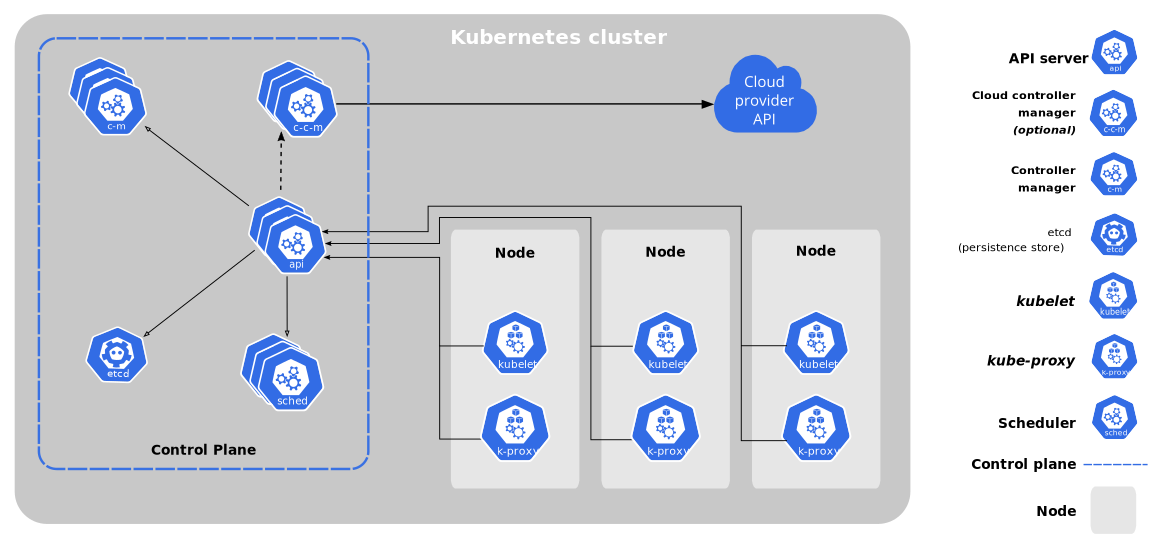
\includegraphics[width=\textwidth]{data/basics/kubernetes-cluster.png}
    \caption{Kubernetes cluster overview \cite{kubernetesdoc2020}}
    \label{fig:kubernetes-cluster}
\end{figure}

Kubernetes offers a very powerful tool for the life cycle of an application in a cluster and paths the way for extensive development of more efficient methods to develop and maintain applications.
\newpage
% Autoscaling
\section{Autoscaling}
The term Autoscaling describes the automatic resource scaling of applications and more detailed microservices \cite{qu2018auto, midigudla2019performance}. As described in the chapter about Kubernetes: autoscaling represents the counter part to the traditional manual scaling of applications. With this method it is possible to allocate more resources for one microservice when it is under especially heavy load or allocate fewer resources when the load gets easier depending on its degree of use in the application by the user.There are in general two types of scaling methods \cite{qu2018auto, midigudla2019performance}: 

\begin{description}
\item[Horizontal] A microservice gets scaled horizontally when its number of instances gets increased or decreased.
\item[Vertical] A microservice gets scaled vertically when the resources of one instance are being increased or decreased.
\end{description}

These two methods describe how a microservice gets scaled but it remains to know when to scale a microservice or the scaling timing. There are existing several approaches: reactive, proactive or even predicted. Furthermore there are several other aspects to pay attention to for example scaling indicators, resource estimation, adaptivity and many more (see figure \ref{fig:autoscaling})\\

\begin{figure}[h]
    \centering
    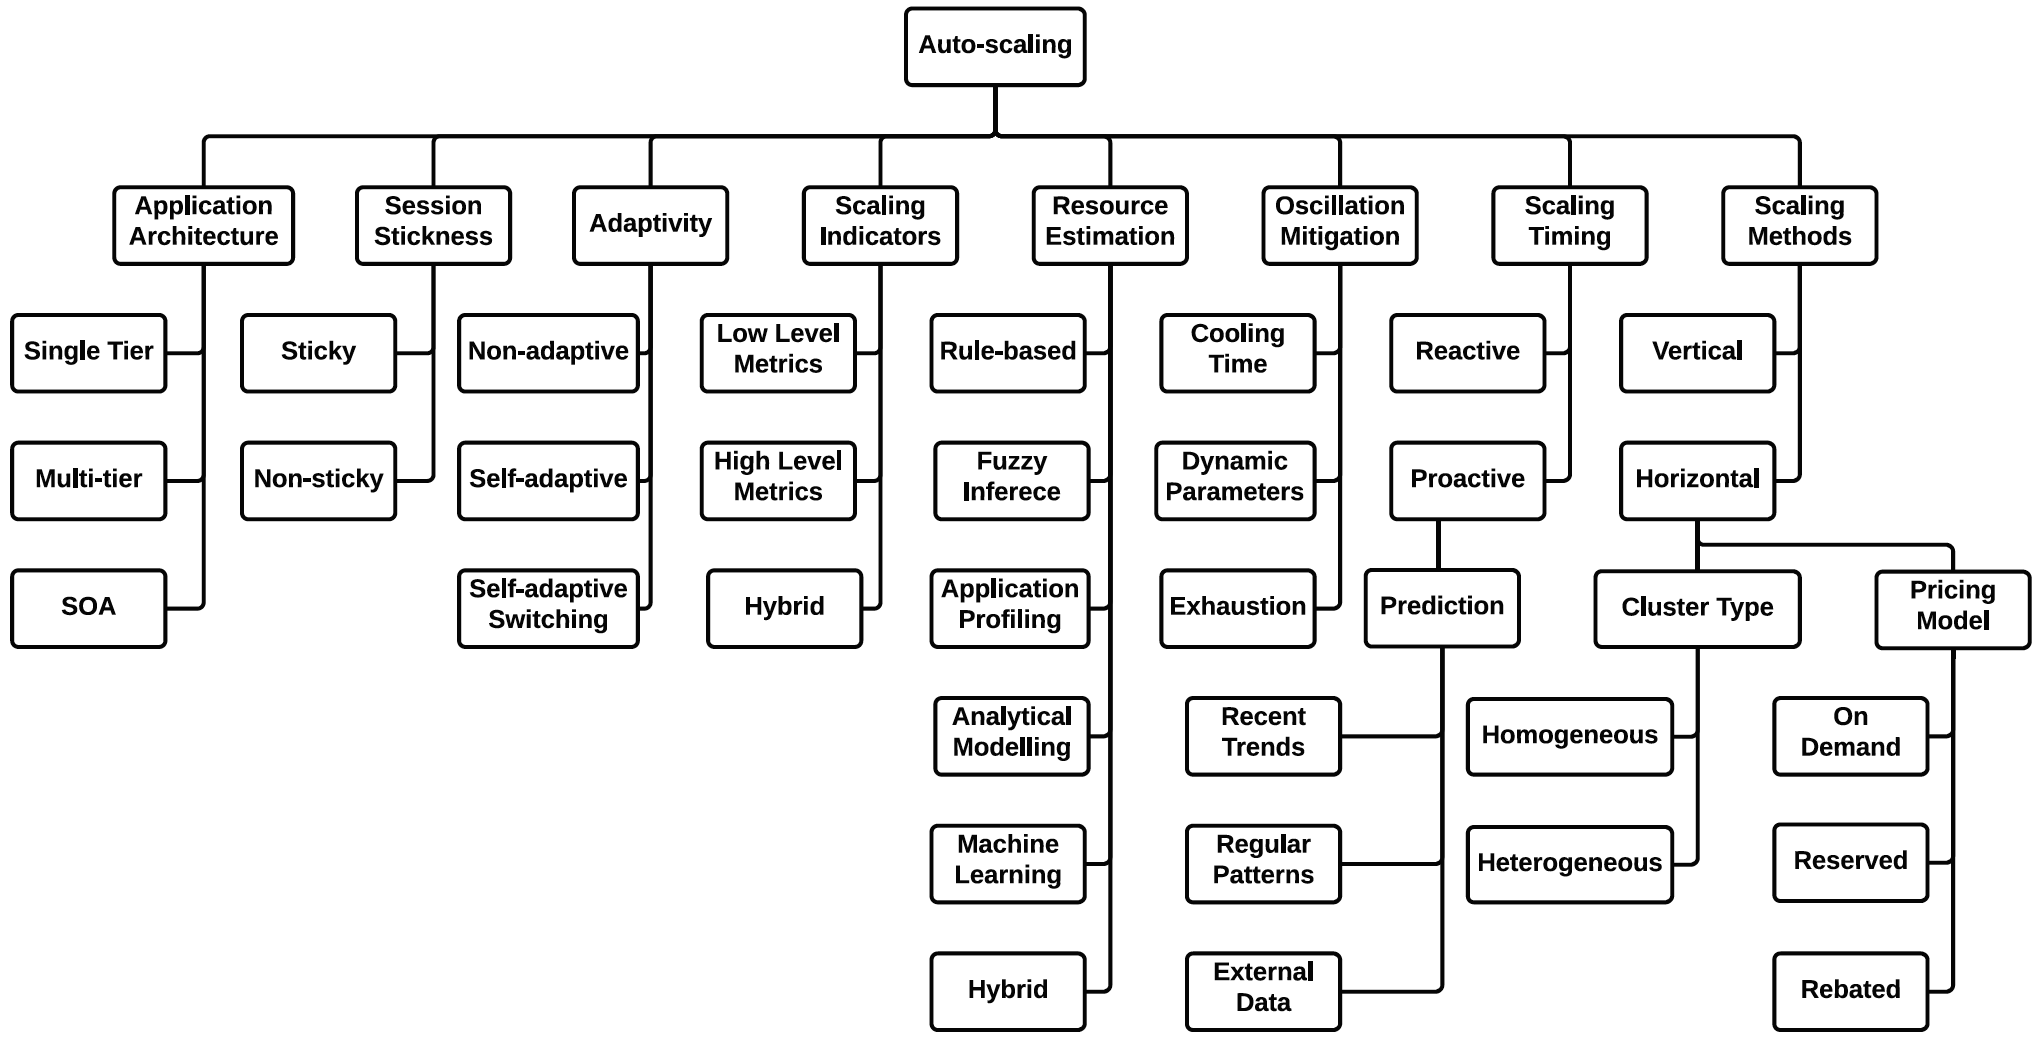
\includegraphics[width=\textwidth]{data/basics/autoscaling.png}
    \caption{Autoscaling taxonomy \cite{qu2018auto}}
    \label{fig:autoscaling}
\end{figure}

The easiest and most common approach to handle all these factors is to define a threshold for certain resources and a scaling method for each microservice manually. When the resource usage of a microservice reaches the set threshold it will scale according to its set configuration.\\
Another way is to use a machine learning algorithm which will be trained to know when and how to scale a certain microservice. This approach will be researched further and implemented in this thesis.
% Support Vector Machines
\section{Machine Learning}
\subsection{Linear Regression}
\subsection{Support Vector Machines}
The Support Vector Machine theory was introduced by Vapnik of the AT\&T Bell Laboratories in 1995 \cite{vapnik1995t}. It describes a supervised machine learning model which is used for classification and regression.\\
The SVM algorithm is designed to find a hyperplane in a $n$-dimensional space which distinguishes data points \cite{awad2015efficient}. In general there are several hyperplanes that are possible, but this algorithm picks the hyperplane with the constraint such that it provides the maximal distance between itself and each class (see figure \ref{fig:svm}). This distance is also called margin, while the nearest data points from each class that determine the maximal margin and therefore influence the hyperplane are called support vectors. The dimension of the hyperplane depends on the number of features $R^{n}$. A hyperplane in for example $R^{2}$ represents a line while it represents a two-dimensional plane in $R^{3}$ \cite{awad2015efficient}.\\
% image begin
\begin{figure}[hp]%
    \centering
    \subfloat[\centering Possible Hyperplanes]{{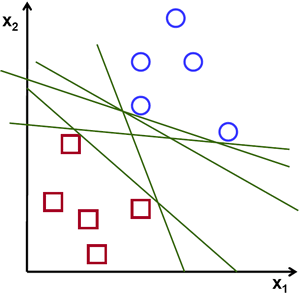
\includegraphics[width=5cm]{data/basics/svm1.png} }}%
    \qquad
    \subfloat[\centering Hyperplane with maximum margin]{{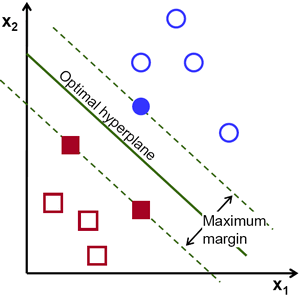
\includegraphics[width=5cm]{data/basics/svm2.png} }}%
    \caption{SVM Hyperplanes \cite{lin2017research}}%
    \label{fig:svm}%
\end{figure}
% image end
In order to handle non-linear problems it uses the kernel trick to transfer the function into higher dimensional feature space \cite{gunn1998support}. Therefore the used kernel function influences the performance of the SVM algorithm significantly and should hence be chosen wisely. The most common kernel functions are "polynomials, radial basis functions and certain
sigmoid functions" \cite{gunn1998support}.\\
\begin{figure}[hp]
\centering
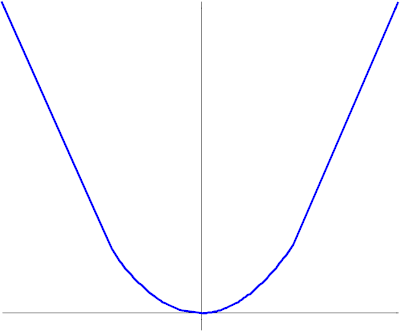
\includegraphics[width=.25\textwidth]{data/basics/svr1.png}\hfill
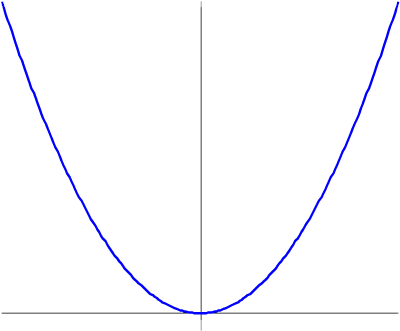
\includegraphics[width=.25\textwidth]{data/basics/svr2.png}\hfill
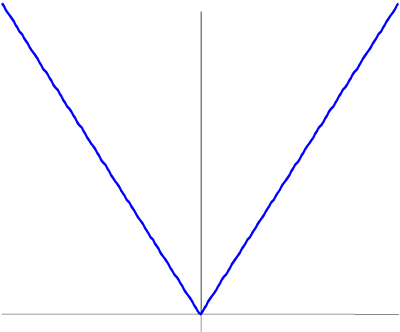
\includegraphics[width=.25\textwidth]{data/basics/svr3.png}
\caption{SVR loss functions \cite{gunn1998support}}
\label{fig:svr}
\end{figure}
Support Vector Machines can, as mentioned before, also be used for regression. In order to realize this, it is necessary to introduce a loss function that includes a distance measure \cite{gunn1998support}. Possible loss functions are for example Quadratic, Laplace or Huber functions (see figure \ref{fig:svr}).
\subsection{Neural Networks}
\newpage
%%%%%%%%%%%%%%%%%%%
% Related Work
%%%%%%%%%%%%%%%%%%%
\chapter{Related Work}
% absolute vs. relative metrics
\newpage
%%%%%%%%%%%%%%%%%%%
% Method
%%%%%%%%%%%%%%%%%%%
\chapter{Method}
\section{Overview}
\section{Environment Setup}
\section{Implementation}
\paragraph{GUI}
\paragraph{Performance Model}
Selection of parameters
* CPU utilization
* CPU share
* Memory utilization
* Memory share
* responds time
\paragraph{Machine Learning Model}
* Support Vector Machine
\paragraph{Control Script}
\section{Extra-P}
\section{Experimentation Methodology}
\newpage
%%%%%%%%%%%%%%%%%%%
% Evaluation
%%%%%%%%%%%%%%%%%%%
\chapter{Evaluation}
\section{Results}
\section{Analysis}
\newpage
%%%%%%%%%%%%%%%%%%%
% Conclusion
%%%%%%%%%%%%%%%%%%%
\chapter{Conclusion}
\section{Summary}
\section{Outlook}
\newpage
%%%%%%%%%%%%%%%%%%%
% Bibliography
%%%%%%%%%%%%%%%%%%%
\renewcommand{\bibname}{References}
\printbibliography

\end{document}
